% Architectures figure — B-grid (2x2, 4x4) and H-grid (2x3, 4x4).
%
% Geometry (local scope coords per core):
%   qubit (row r, col c): x = c*0.4, y = -r*0.4   (row 0 = top)
%   core box: (-0.2, -1.4) rectangle (1.4, 0.2)
%   core-to-core spacing: 2.1 in x and y
%
% Comm ports (teal) per core — B-grid:
%   C0: (r1,c3)=(1.2,-0.4) to C1;  (r3,c1)=(0.4,-1.2) to C2
%   C1: (r1,c0)=(0,-0.4)   to C0;  (r3,c2)=(0.8,-1.2) to C3
%   C2: (r0,c1)=(0.4,0)    to C0;  (r2,c3)=(1.2,-0.8) to C3
%   C3: (r0,c2)=(0.8,0)    to C1;  (r2,c0)=(0,-0.8)   to C2
%
% Comm ports — H-grid (C1,C4 have 3 ports):
%   C0: (r1,c3)=(1.2,-0.4) to C1;  (r3,c1)=(0.4,-1.2) to C3
%   C1: (r1,c0)=(0,-0.4)   to C0;  (r1,c3)=(1.2,-0.4) to C2;  (r3,c2)=(0.8,-1.2) to C4
%   C2: (r1,c0)=(0,-0.4)   to C1;  (r3,c2)=(0.8,-1.2) to C5
%   C3: (r0,c1)=(0.4,0)    to C0;  (r2,c3)=(1.2,-0.8) to C4
%   C4: (r0,c1)=(0.4,0)    to C1;  (r2,c0)=(0,-0.8)   to C3;  (r2,c3)=(1.2,-0.8) to C5
%   C5: (r0,c2)=(0.8,0)    to C2;  (r2,c0)=(0,-0.8)   to C4
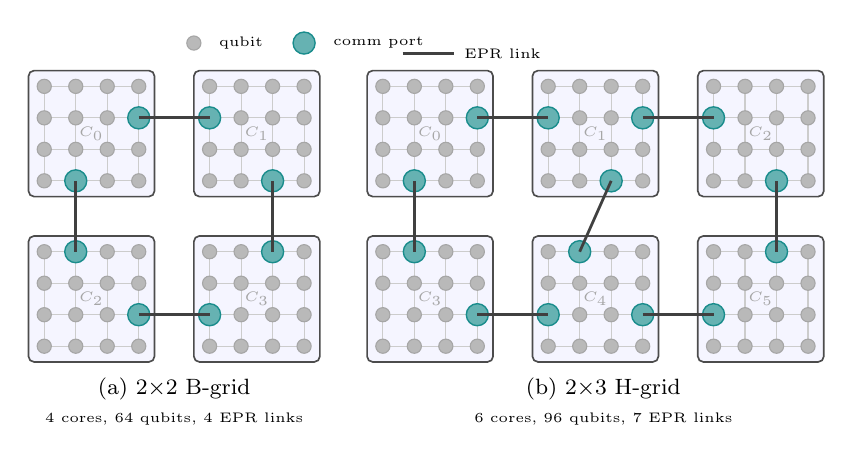
\begin{tikzpicture}[
  every node/.style={font=\scriptsize},
  dot/.style  ={circle, fill=gray!55,  draw=gray!70,  minimum size=1.8mm, inner sep=0pt},
  cport/.style={circle, fill=teal!60,  draw=teal!90,  minimum size=2.8mm, inner sep=0pt, line width=0.5pt},
  cbox/.style ={draw=black!70, rounded corners=2pt, fill=blue!4, line width=0.6pt},
  ie/.style   ={draw=gray!40, line width=0.4pt},
  cl/.style   ={draw=black!75, line width=1.0pt},
]

%% ─── Helper: draw one 4×4 core at given shift ────────────────────────────────
%% Called as:  \begin{scope}[shift={(...)}] \CoreGrid \end{scope}
%% then comm ports drawn explicitly in each core's scope.
\tikzset{CoreGrid/.style={}}   % placeholder; we draw inline per core

%% ═══════════════════════════════════════════════════════════════════════════
%% B-GRID  (2×2 array of 4×4 cores)
%% Cores: C0 top-left, C1 top-right, C2 bottom-left, C3 bottom-right
%% ═══════════════════════════════════════════════════════════════════════════

%% ── C0 (shift 0,0) ──────────────────────────────────────────────────────────
\begin{scope}[shift={(0,0)}]
  \draw[cbox] (-0.2,-1.4) rectangle (1.4,0.2);
  \foreach \r in {0,1,2,3}{\foreach \dc in {0,1,2}{
    \draw[ie]({\dc*0.4},{-\r*0.4})--({\dc*0.4+0.4},{-\r*0.4});}}
  \foreach \c in {0,1,2,3}{\foreach \dr in {0,1,2}{
    \draw[ie]({\c*0.4},{-\dr*0.4})--({\c*0.4},{-\dr*0.4-0.4});}}
  \foreach \r in {0,1,2,3}{\foreach \c in {0,1,2,3}{
    \node[dot] at ({\c*0.4},{-\r*0.4}) {};}}
  \node[cport] at (1.2,-0.4) {};   % r1c3 -> C1
  \node[cport] at (0.4,-1.2) {};   % r3c1 -> C2
  \node[font=\tiny,gray!70] at (0.6,-0.6) {$C_0$};
\end{scope}

%% ── C1 (shift 2.1,0) ────────────────────────────────────────────────────────
\begin{scope}[shift={(2.1,0)}]
  \draw[cbox] (-0.2,-1.4) rectangle (1.4,0.2);
  \foreach \r in {0,1,2,3}{\foreach \dc in {0,1,2}{
    \draw[ie]({\dc*0.4},{-\r*0.4})--({\dc*0.4+0.4},{-\r*0.4});}}
  \foreach \c in {0,1,2,3}{\foreach \dr in {0,1,2}{
    \draw[ie]({\c*0.4},{-\dr*0.4})--({\c*0.4},{-\dr*0.4-0.4});}}
  \foreach \r in {0,1,2,3}{\foreach \c in {0,1,2,3}{
    \node[dot] at ({\c*0.4},{-\r*0.4}) {};}}
  \node[cport] at (0,   -0.4) {};   % r1c0 -> C0
  \node[cport] at (0.8, -1.2) {};   % r3c2 -> C3
  \node[font=\tiny,gray!70] at (0.6,-0.6) {$C_1$};
\end{scope}

%% ── C2 (shift 0,-2.1) ───────────────────────────────────────────────────────
\begin{scope}[shift={(0,-2.1)}]
  \draw[cbox] (-0.2,-1.4) rectangle (1.4,0.2);
  \foreach \r in {0,1,2,3}{\foreach \dc in {0,1,2}{
    \draw[ie]({\dc*0.4},{-\r*0.4})--({\dc*0.4+0.4},{-\r*0.4});}}
  \foreach \c in {0,1,2,3}{\foreach \dr in {0,1,2}{
    \draw[ie]({\c*0.4},{-\dr*0.4})--({\c*0.4},{-\dr*0.4-0.4});}}
  \foreach \r in {0,1,2,3}{\foreach \c in {0,1,2,3}{
    \node[dot] at ({\c*0.4},{-\r*0.4}) {};}}
  \node[cport] at (0.4,  0)    {};   % r0c1 -> C0
  \node[cport] at (1.2, -0.8) {};   % r2c3 -> C3
  \node[font=\tiny,gray!70] at (0.6,-0.6) {$C_2$};
\end{scope}

%% ── C3 (shift 2.1,-2.1) ─────────────────────────────────────────────────────
\begin{scope}[shift={(2.1,-2.1)}]
  \draw[cbox] (-0.2,-1.4) rectangle (1.4,0.2);
  \foreach \r in {0,1,2,3}{\foreach \dc in {0,1,2}{
    \draw[ie]({\dc*0.4},{-\r*0.4})--({\dc*0.4+0.4},{-\r*0.4});}}
  \foreach \c in {0,1,2,3}{\foreach \dr in {0,1,2}{
    \draw[ie]({\c*0.4},{-\dr*0.4})--({\c*0.4},{-\dr*0.4-0.4});}}
  \foreach \r in {0,1,2,3}{\foreach \c in {0,1,2,3}{
    \node[dot] at ({\c*0.4},{-\r*0.4}) {};}}
  \node[cport] at (0.8,  0)    {};   % r0c2 -> C1
  \node[cport] at (0,   -0.8) {};   % r2c0 -> C2
  \node[font=\tiny,gray!70] at (0.6,-0.6) {$C_3$};
\end{scope}

%% ── B-grid inter-core links ──────────────────────────────────────────────────
\draw[cl] (1.2,-0.4)  -- (2.1,-0.4);    % C0(r1c3) -- C1(r1c0)
\draw[cl] (0.4,-1.2)  -- (0.4,-2.1);    % C0(r3c1) -- C2(r0c1)
\draw[cl] (2.9,-1.2)  -- (2.9,-2.1);    % C1(r3c2) -- C3(r0c2)
\draw[cl] (1.2,-2.9)  -- (2.1,-2.9);    % C2(r2c3) -- C3(r2c0)

%% ── B-grid label ─────────────────────────────────────────────────────────────
\node[font=\footnotesize, align=center] at (1.65,-4)
  {(a)~$2{\times}2$ B-grid\\[0.5pt]{\tiny 4 cores,\ 64 qubits,\ 4 EPR links}};


%% ═══════════════════════════════════════════════════════════════════════════
%% H-GRID  (2×3 array of 4×4 cores)    x-offset = 4.3
%% Cores: C0 top-left, C1 top-mid, C2 top-right,
%%        C3 bot-left, C4 bot-mid,  C5 bot-right
%% ═══════════════════════════════════════════════════════════════════════════
\def\hx{4.3}

%% ── C0 (shift \hx,0) ────────────────────────────────────────────────────────
\begin{scope}[shift={(\hx,0)}]
  \draw[cbox] (-0.2,-1.4) rectangle (1.4,0.2);
  \foreach \r in {0,1,2,3}{\foreach \dc in {0,1,2}{
    \draw[ie]({\dc*0.4},{-\r*0.4})--({\dc*0.4+0.4},{-\r*0.4});}}
  \foreach \c in {0,1,2,3}{\foreach \dr in {0,1,2}{
    \draw[ie]({\c*0.4},{-\dr*0.4})--({\c*0.4},{-\dr*0.4-0.4});}}
  \foreach \r in {0,1,2,3}{\foreach \c in {0,1,2,3}{
    \node[dot] at ({\c*0.4},{-\r*0.4}) {};}}
  \node[cport] at (1.2,-0.4) {};   % r1c3 -> C1
  \node[cport] at (0.4,-1.2) {};   % r3c1 -> C3
  \node[font=\tiny,gray!70] at (0.6,-0.6) {$C_0$};
\end{scope}

%% ── C1 (shift \hx+2.1, 0) ───────────────────────────────────────────────────
\begin{scope}[shift={(\hx+2.1,0)}]
  \draw[cbox] (-0.2,-1.4) rectangle (1.4,0.2);
  \foreach \r in {0,1,2,3}{\foreach \dc in {0,1,2}{
    \draw[ie]({\dc*0.4},{-\r*0.4})--({\dc*0.4+0.4},{-\r*0.4});}}
  \foreach \c in {0,1,2,3}{\foreach \dr in {0,1,2}{
    \draw[ie]({\c*0.4},{-\dr*0.4})--({\c*0.4},{-\dr*0.4-0.4});}}
  \foreach \r in {0,1,2,3}{\foreach \c in {0,1,2,3}{
    \node[dot] at ({\c*0.4},{-\r*0.4}) {};}}
  \node[cport] at (0,   -0.4) {};   % r1c0 -> C0
  \node[cport] at (1.2, -0.4) {};   % r1c3 -> C2
  \node[cport] at (0.8, -1.2) {};   % r3c2 -> C4
  \node[font=\tiny,gray!70] at (0.6,-0.6) {$C_1$};
\end{scope}

%% ── C2 (shift \hx+4.2, 0) ───────────────────────────────────────────────────
\begin{scope}[shift={(\hx+4.2,0)}]
  \draw[cbox] (-0.2,-1.4) rectangle (1.4,0.2);
  \foreach \r in {0,1,2,3}{\foreach \dc in {0,1,2}{
    \draw[ie]({\dc*0.4},{-\r*0.4})--({\dc*0.4+0.4},{-\r*0.4});}}
  \foreach \c in {0,1,2,3}{\foreach \dr in {0,1,2}{
    \draw[ie]({\c*0.4},{-\dr*0.4})--({\c*0.4},{-\dr*0.4-0.4});}}
  \foreach \r in {0,1,2,3}{\foreach \c in {0,1,2,3}{
    \node[dot] at ({\c*0.4},{-\r*0.4}) {};}}
  \node[cport] at (0,   -0.4) {};   % r1c0 -> C1
  \node[cport] at (0.8, -1.2) {};   % r3c2 -> C5
  \node[font=\tiny,gray!70] at (0.6,-0.6) {$C_2$};
\end{scope}

%% ── C3 (shift \hx, -2.1) ────────────────────────────────────────────────────
\begin{scope}[shift={(\hx,-2.1)}]
  \draw[cbox] (-0.2,-1.4) rectangle (1.4,0.2);
  \foreach \r in {0,1,2,3}{\foreach \dc in {0,1,2}{
    \draw[ie]({\dc*0.4},{-\r*0.4})--({\dc*0.4+0.4},{-\r*0.4});}}
  \foreach \c in {0,1,2,3}{\foreach \dr in {0,1,2}{
    \draw[ie]({\c*0.4},{-\dr*0.4})--({\c*0.4},{-\dr*0.4-0.4});}}
  \foreach \r in {0,1,2,3}{\foreach \c in {0,1,2,3}{
    \node[dot] at ({\c*0.4},{-\r*0.4}) {};}}
  \node[cport] at (0.4,  0)    {};   % r0c1 -> C0
  \node[cport] at (1.2, -0.8) {};   % r2c3 -> C4
  \node[font=\tiny,gray!70] at (0.6,-0.6) {$C_3$};
\end{scope}

%% ── C4 (shift \hx+2.1, -2.1) ────────────────────────────────────────────────
\begin{scope}[shift={(\hx+2.1,-2.1)}]
  \draw[cbox] (-0.2,-1.4) rectangle (1.4,0.2);
  \foreach \r in {0,1,2,3}{\foreach \dc in {0,1,2}{
    \draw[ie]({\dc*0.4},{-\r*0.4})--({\dc*0.4+0.4},{-\r*0.4});}}
  \foreach \c in {0,1,2,3}{\foreach \dr in {0,1,2}{
    \draw[ie]({\c*0.4},{-\dr*0.4})--({\c*0.4},{-\dr*0.4-0.4});}}
  \foreach \r in {0,1,2,3}{\foreach \c in {0,1,2,3}{
    \node[dot] at ({\c*0.4},{-\r*0.4}) {};}}
  \node[cport] at (0.4,  0)    {};   % r0c1 -> C1 (note: col=1, staggered)
  \node[cport] at (0,   -0.8) {};   % r2c0 -> C3
  \node[cport] at (1.2, -0.8) {};   % r2c3 -> C5
  \node[font=\tiny,gray!70] at (0.6,-0.6) {$C_4$};
\end{scope}

%% ── C5 (shift \hx+4.2, -2.1) ────────────────────────────────────────────────
\begin{scope}[shift={(\hx+4.2,-2.1)}]
  \draw[cbox] (-0.2,-1.4) rectangle (1.4,0.2);
  \foreach \r in {0,1,2,3}{\foreach \dc in {0,1,2}{
    \draw[ie]({\dc*0.4},{-\r*0.4})--({\dc*0.4+0.4},{-\r*0.4});}}
  \foreach \c in {0,1,2,3}{\foreach \dr in {0,1,2}{
    \draw[ie]({\c*0.4},{-\dr*0.4})--({\c*0.4},{-\dr*0.4-0.4});}}
  \foreach \r in {0,1,2,3}{\foreach \c in {0,1,2,3}{
    \node[dot] at ({\c*0.4},{-\r*0.4}) {};}}
  \node[cport] at (0.8,  0)    {};   % r0c2 -> C2
  \node[cport] at (0,   -0.8) {};   % r2c0 -> C4
  \node[font=\tiny,gray!70] at (0.6,-0.6) {$C_5$};
\end{scope}

%% ── H-grid inter-core links ──────────────────────────────────────────────────
% Global coords = local scope coords + shift
% C0@(\hx,0): C0(r1c3)=(\hx+1.2,-0.4)  C0(r3c1)=(\hx+0.4,-1.2)
% C1@(\hx+2.1,0): C1(r1c0)=(\hx+2.1,-0.4)  C1(r1c3)=(\hx+3.3,-0.4)  C1(r3c2)=(\hx+2.9,-1.2)
% C2@(\hx+4.2,0): C2(r1c0)=(\hx+4.2,-0.4)  C2(r3c2)=(\hx+5.0,-1.2)
% C3@(\hx,-2.1):  C3(r0c1)=(\hx+0.4,-2.1)  C3(r2c3)=(\hx+1.2,-2.9)
% C4@(\hx+2.1,-2.1): C4(r0c1)=(\hx+2.5,-2.1)  C4(r2c0)=(\hx+2.1,-2.9)  C4(r2c3)=(\hx+3.3,-2.9)
% C5@(\hx+4.2,-2.1): C5(r0c2)=(\hx+5.0,-2.1)  C5(r2c0)=(\hx+4.2,-2.9)
\draw[cl] (\hx+1.2,-0.4) -- (\hx+2.1,-0.4);   % C0(r1c3) -- C1(r1c0)
\draw[cl] (\hx+3.3,-0.4) -- (\hx+4.2,-0.4);   % C1(r1c3) -- C2(r1c0)
\draw[cl] (\hx+0.4,-1.2) -- (\hx+0.4,-2.1);   % C0(r3c1) -- C3(r0c1)
\draw[cl] (\hx+2.9,-1.2) -- (\hx+2.5,-2.1);   % C1(r3c2) -- C4(r0c1)  [staggered]
\draw[cl] (\hx+5.0,-1.2) -- (\hx+5.0,-2.1);   % C2(r3c2) -- C5(r0c2)
\draw[cl] (\hx+1.2,-2.9) -- (\hx+2.1,-2.9);   % C3(r2c3) -- C4(r2c0)
\draw[cl] (\hx+3.3,-2.9) -- (\hx+4.2,-2.9);   % C4(r2c3) -- C5(r2c0)

%% ── H-grid label ─────────────────────────────────────────────────────────────
\node[font=\footnotesize, align=center] at (\hx+2.8,-4)
  {(b)~$2{\times}3$ H-grid\\[0.5pt]{\tiny 6 cores,\ 96 qubits,\ 7 EPR links}};

%% ── Legend ───────────────────────────────────────────────────────────────────
\node[dot,   label={[font=\tiny,xshift=1mm]right:qubit}]   at (1.9, 0.55) {};
\node[cport, label={[font=\tiny,xshift=1mm]right:comm port}] at (3.3, 0.55) {};
\draw[cl] (4.55,0.42) -- (5.2,0.42)
  node[right, font=\tiny] {EPR link};

\end{tikzpicture}
